\chapter{Desenvolvimento}
\label{cap:03}

\section{MMF}

O MMF, é um framework modular para pesquisa de visão e linguagem multimodal de código aberto criado pelo Facebook AI Research (FAIR). É considerado o estado da arte (state-of-the-art) desse seguimento, onde foi utilizado como referência para desenvolver projetos como o Visualbert.

Já o Detectron2 é uma plataforma também de código aberto para detecção de objetos, segmentação e outras tarefas de reconhecimento visual. Também é considerado o estado da arte em detecção e segmentação, onde oferece suporte a vários projetos de pesquisa de visão computacional.

PyTorch é uma biblioteca de aprendizado de máquina em código aberto usada para implementações de aprendizado profundo, como visão computacional (usando TorchVision) e processamento de linguagem natural

\begin{figure*}[!htbp]
	\centering
	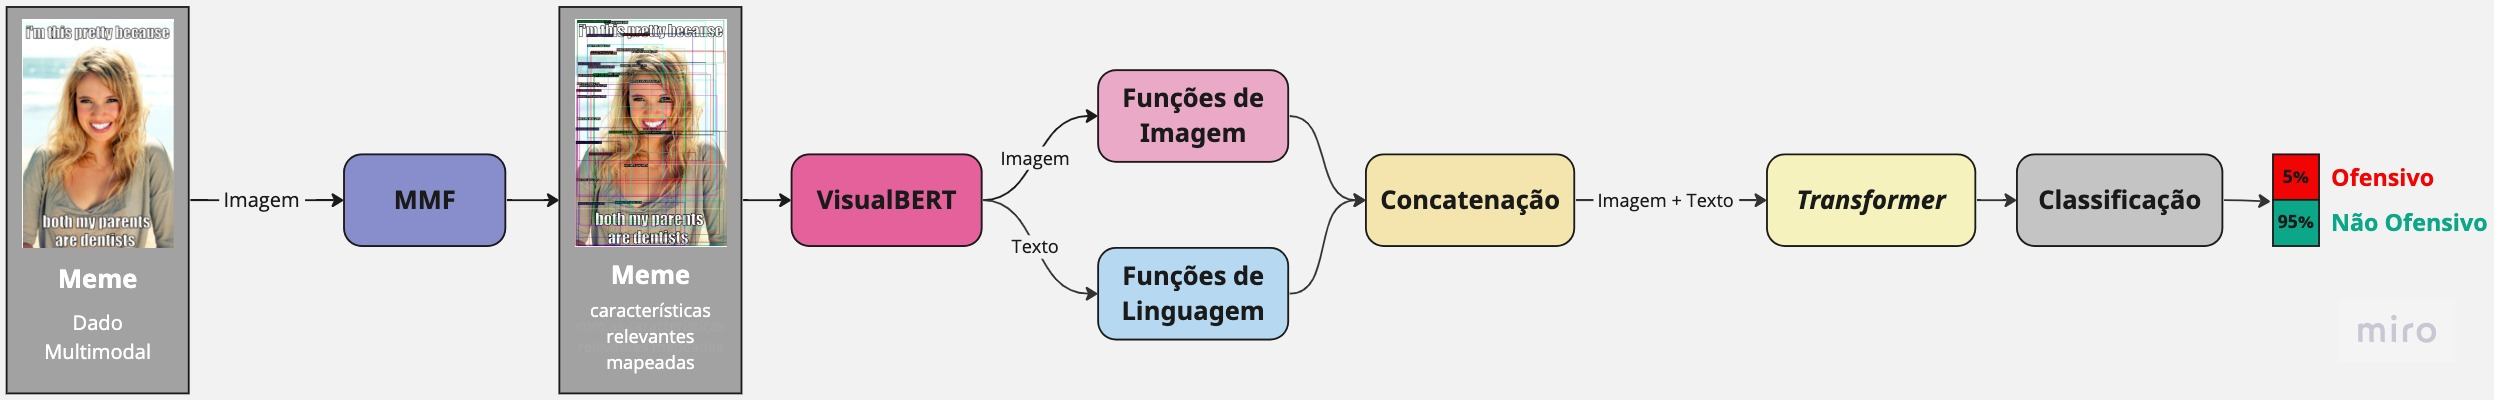
\includegraphics[scale=0.18]{imagens/diagrama.jpeg}
    \caption {Arquitetura da Proposta de Desenvolvimento.}
\end{figure*}
